\subsection{Spawning of an agent}
\label{sec:spawning}

TODO what is spawning

The second outside interaction is required to spawn the agent. To spawn an agent, the user must send an HTTP Post request to the `/api/v1/servers/\{dslId\}/start' endpoint of the Core server. The \ref{fig:start1} figure shows how the service layer of the Core server handles the request.

\begin{figure}[h]
    \centering
    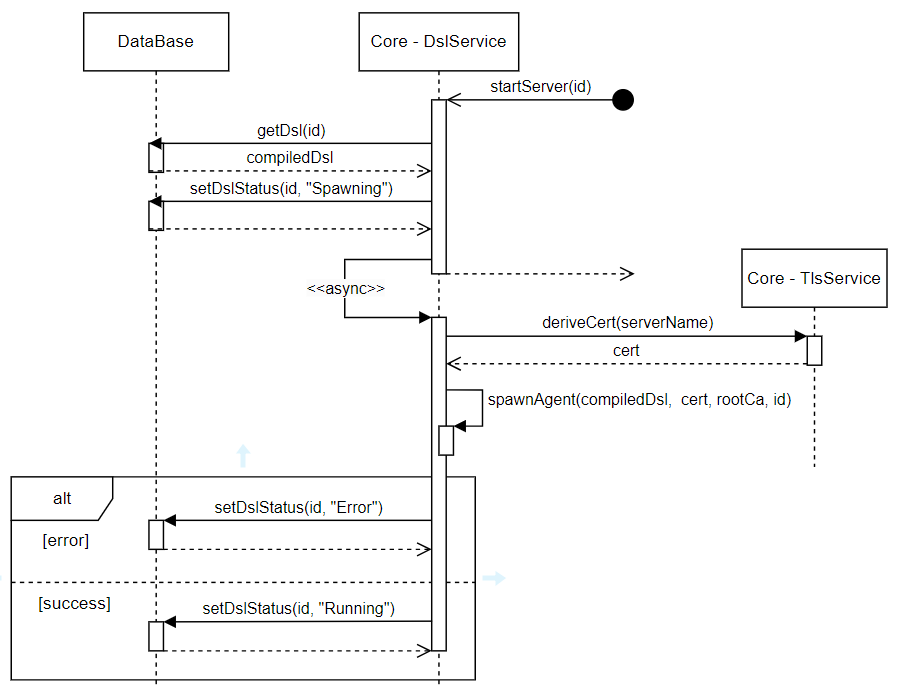
\includegraphics[width=130mm, keepaspectratio]{seq5.png}
    \caption{Spawning of an agent}
    \label{fig:start1}
\end{figure}

First, the compiled script is loaded from the database. Secondly, the status of the DSL script is set to `Spawning'. The rest is done on another thread, and the `startServer' function returns.

All agents use HTTPS, so they require a TLS certificate, which can be requested from the TlsService.
After a new certificate is created, the next step is to execute the compiled script, to extract information, such as the name of the \emph{ClusterRole}, or the webhook configurations, all of which are required during the spawning of the agent.

In the \ref{fig:start1} diagram, the steps of spawning an agent are not detailed; instead, these steps are abstracted by the `spawnAgent' function. The \ref{code:start2} pseudocode better summarizes the steps of the `spawnAgent' function than a sequence diagram.

\begin{lstlisting}[caption={Spawning of an agent},language=Kotlin,label=code:start2]
val server = executeScript(compiledDsl)

k8s.create(Secret(rootCa, certificates))

val dep = Deployment(server)
val svc = Service(server)
if (server.hasClusterRole() == true) {
    val sa = ServiceAccount(server)
    val crb = ClusterRoleBinding(server)
    k8s.create(sa)
    k8s.create(crb)
    dep.serviceAccountName = sa.name
}
k8s.create(dep)
k8s.create(svc)
...
\end{lstlisting}

First, a Kubernetes \emph{Secret} resource is created with the certificates and keys needed for the Agent. This will be mounted to the \emph{Deployment}.
After that, a \emph{Deployment} and a \emph{Service} object are created locally using the configuration from the server object. If the server has the `clusterRole' keyword set, a \emph{ServiceAccount} and a \emph{ClusterRoleBinding} are created as well, and the previously created \emph{Deployment} is set to use the \emph{ServiceAccount}. After that, the \emph{Deployment} and the \emph{Service} are created on the cluster too.

The creation of the \emph{Deployment} does not imply that the agent is ready to serve requests, so the spawning has to wait for the agent to become available. The \emph{MutatingWebhookConfiguration} should not be created before the agent can serve requests because that would result in an unstable state, where an admission webhook has no actual server implementing it. The details of how an agent actually starts up are described in the next section. For now, let's focus on what's happening inside the Core component.

The \ref{code:start3} pseudocode shows how the startup of the agent is awaited, and what additional steps are done.

\begin{lstlisting}[caption={Spawning of an agent},language=Kotlin,label=code:start3]
...
try {
    k8s.waitUntilAvailable(dep)
    success = true
} catch (e: TimeoutException) {
    doRollback()
    success = false
}
        
if (success) {
    k8s.create(MutatingWebhookConfiguration(server, rootCa))
    setDslStatus(id, "Running")
} else {
    setDslStatus(id, "Error")
}
\end{lstlisting}

If the agent becomes available before the timeout, the \emph{MutatingWebhookConfiguration} is created too. Otherwise, a rollback is performed, deleting all the previously created resources.

Finally, the status of the agent is updated in the database.

Note: Both start and delete operations on an agent must be atomic. Given that an agent is composed of multiple Kubernetes resources, it is crucial that during creation, all components are created without errors, and during deletion, all components are destroyed. The Core component is implemented to ensure this atomic behavior.
